\documentclass[aspectratio=169, 11pt]{beamer}

% ── Configuración de idioma y fuentes ──
\usepackage[spanish, es-noshorthands]{babel}
\usepackage[utf8]{inputenc}
\usepackage[T1]{fontenc}
\usepackage{lmodern}
\usepackage{microtype}
\usepackage{graphicx}

% ── Configuración del tema Beamer ──
\usetheme{Madrid}
\usecolortheme{default}

% ── Colores corporativos (SHCP - UPIT / VINO) ──
\definecolor{vino}{HTML}{6E152E}
\definecolor{vinoDark}{HTML}{4B1A28}
\definecolor{vinoLite}{HTML}{b84a6b}

% Aplicar colores al tema de la presentación
\setbeamercolor{palette primary}{bg=vino,fg=white}
\setbeamercolor{palette secondary}{bg=vinoDark,fg=white}
\setbeamercolor{palette tertiary}{bg=vinoLite,fg=white}
\setbeamercolor{structure}{fg=vino}
\setbeamercolor{title}{bg=vino,fg=white}
\setbeamercolor{frametitle}{bg=vino,fg=white}
\setbeamercolor{item projected}{bg=vino,fg=white}
\setbeamercolor{block title}{bg=vino,fg=white}
\setbeamercolor{block body}{bg=vino!6,fg=black}

% Eliminar iconos de navegación abajo
\setbeamertemplate{navigation symbols}{}

% ── Datos de la Portada ──
\title[Conciliador v6.6]{Conciliador de Cotizaciones v6.6}
\subtitle{Extracción inteligente de presupuestos, auto-detección de secciones y validación normativa EFIDEPORTE}
\author[SHCP - UPIT]{SHCP - UPIT}
\date{\today}

\begin{document}

% ── Diapositiva 1: Portada ──
\begin{frame}
    \titlepage
\end{frame}

% ── Diapositiva 2: El Problema Actual ──
\begin{frame}{El Problema Actual}
    \begin{itemize}
        \item \textbf{Procesos Manuales Lentos:} La transcripción de datos económicos desde archivos PDF a hojas de Excel consume horas de revisión por expediente.
        \item \textbf{Expedientes Consolidados en PDF Único:} Los proyectos reúnen presupuesto global, decenas de cotizaciones, cartas manifiesto y anexos escaneados en cientos de páginas.
        \item \textbf{Riesgo de Errores Humanos:} El tipeo manual de cifras largas, descuentos e IVA provoca discrepancias en presupuestos de obra o equipamiento.
        \item \textbf{Falta de Estandarización y Escaneos Difíciles:} Cada proveedor usa formatos distintos, tipografías pequeñas, fondos oscuros o capas OCR incrustadas deficientes.
        \item \textbf{Cálculos Cambiarios Tediosos:} Las cotizaciones en USD, EUR o CAD exigen consultar manualmente el tipo de cambio oficial de Banxico por fecha de emisión.
    \end{itemize}
\end{frame}

% ── Diapositiva 3: Nuestra Solución ──
\begin{frame}{Nuestra Solución: Conciliador de Cotizaciones v6.6}
    Aplicación de escritorio \textbf{nativa para Windows} (PyQt6) distribuida como ejecutable único portable (\texttt{Conciliador.exe}), sin instalación ni servidor web.

    \vspace{0.4cm}
    \begin{columns}[T]
        \column{0.54\textwidth}
        \textbf{¿Qué logra en la versión 6.6?}
        \begin{itemize}
            \item Segmenta automáticamente expedientes completos en un solo PDF en segundos.
            \item Extrae montos, fechas, divisas e IVA con motor multinivel y OCR avanzado de doble pasada.
            \item Audita en vivo los 7 Lineamientos normativos EFIDEPORTE antes de exportar.
            \item Genera reportes Excel corporativos y guarda sesiones completas en archivos portables \texttt{.cshcp}.
        \end{itemize}

        \column{0.44\textwidth}
        \begin{center}
            \fcolorbox{vino}{vino!10}{
                \parbox{0.9\linewidth}{
                    \centering
                    \textbf{\color{vino}Impacto Operativo}\\[6pt]
                    \normalsize
                    Reducción superior al \textbf{80\%} en tiempo de conciliación manual.\\[6pt]
                    \small Soporte hasta \textbf{500+ secciones} por expediente y validación automática de totales con texto en letra.
                }
            }
        \end{center}
    \end{columns}
\end{frame}

% ── Diapositiva 4: Características Técnicas Principales ──
\begin{frame}{Características Técnicas Principales}
    \begin{enumerate}
        \item \textbf{5 Estrategias + OCR Avanzado de Doble Pasada:} Tablas nativas, triangulación matemática ($Q \times PU \approx T$), detección de capas OCR corruptas (p.\ ej.\ \textit{iLovePDF}), inversión adaptativa de fondos oscuros, escalado automático PyTesseract $\rightarrow$ RapidOCR y opción \textit{Forzar OCR de alta precisión}.
        \item \textbf{API Banxico Integrada y en Caliente:} Consulta automática de USD, EUR y CAD por fecha de emisión (Serie Banxico) y botón \textbf{Aplicar} para actualizar divisas sin sobrescribir ediciones manuales.
        \item \textbf{Proyectos Portables (\texttt{.cshcp}) y Trazabilidad MD5:} Encapsula PDFs, secciones, parámetros normativos, estado OCR y tabla en un solo archivo reutilizable con sello de integridad MD5.
        \item \textbf{Exportación Inteligente a Excel:} Reportes \texttt{.xlsx} corporativos con fórmulas vivas de Subtotal, IVA, Total y Diferencias en formato \textbf{Tamaño Carta, Horizontal} listo para imprimir.
    \end{enumerate}
\end{frame}

% ── Diapositiva 5: Auto-detección de Secciones (NUEVA) ──
\begin{frame}{Auto-detección de Secciones (Expedientes en PDF Único)}
    \begin{columns}[c]
        \column{0.42\textwidth}
        \small
        \textbf{Segmentación en 1 clic:}
        \begin{itemize}
            \setlength{\itemsep}{4pt}
            \item Con un PDF único cargado se habilita \textbf{Auto-detectar secciones}.
            \item Combina marcadores PDF, encabezados, títulos desbordados y OCR ligero en escaneos.
            \item \textbf{Filtro inteligente:} Desmarca resúmenes financieros, oficios, croquis y cartas EFIDEPORTE (Anexo 29 y 34--40).
            \item \textbf{Revisión en vivo:} Edita rangos, confirma casillas y previsualiza cada corte en el visor.
        \end{itemize}

        \column{0.56\textwidth}
        \centering
        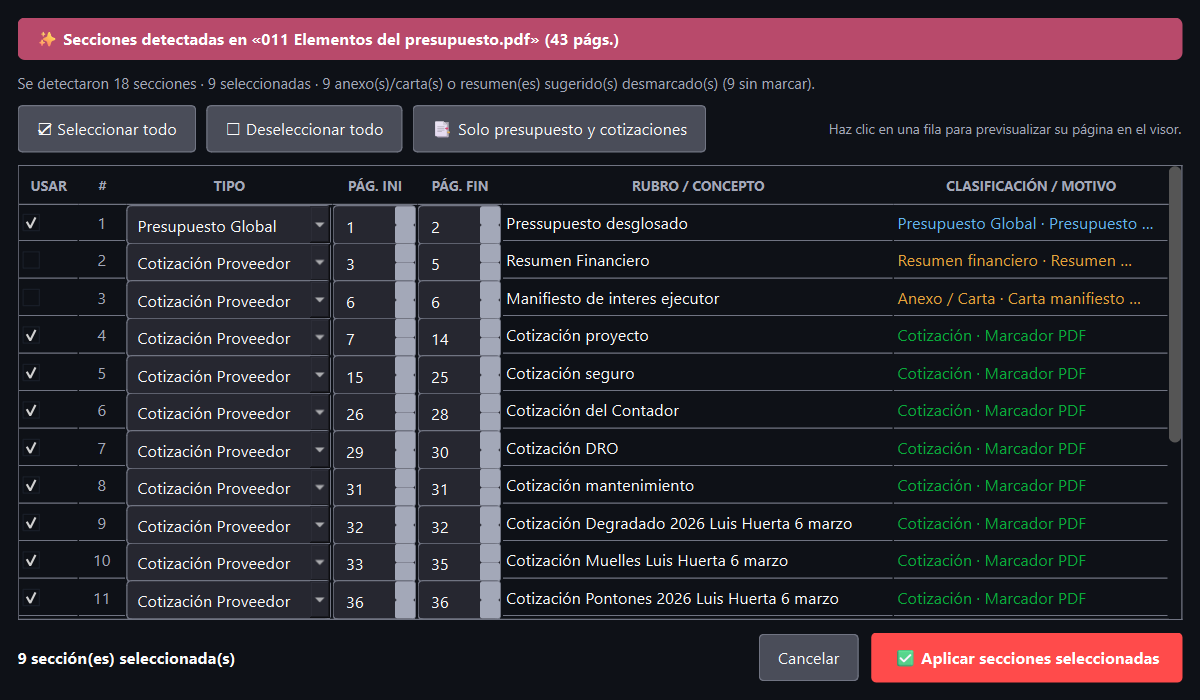
\includegraphics[width=\linewidth, height=0.68\textheight, keepaspectratio]{../images/09_auto_detectar_dialogo.png}
    \end{columns}
\end{frame}

% ── Diapositiva 6: Flujo de Trabajo e Interfaz Renovada ──
\begin{frame}{Flujo de Trabajo e Interfaz Renovada}
    \begin{center}
        \scriptsize
        \colorbox{vino}{\color{white}\textbf{1. Cargar PDF(s)}} $\rightarrow$
        \colorbox{vino}{\color{white}\textbf{2. Auto-detectar / Config.}} $\rightarrow$
        \colorbox{vino}{\color{white}\textbf{3. Extraer Montos}} $\rightarrow$
        \colorbox{vino}{\color{white}\textbf{4. Validar}} $\rightarrow$
        \colorbox{vino}{\color{white}\textbf{5. Exportar}}
    \end{center}
    \vspace{0.15cm}
    \begin{columns}[c]
        \column{0.41\textwidth}
        \small
        \begin{itemize}
            \setlength{\itemsep}{4pt}
            \item \textbf{Panel fijo (310 px):} Sin barra horizontal ni recortes; tarjetas con encabezados dinámicos por píxeles.
            \item \textbf{Visor PDF sincronizado:} Zoom, paneo, rotación y etiqueta de sección activa.
            \item \textbf{Recálculo en vivo:} Editar cantidad, precio, IVA o divisa actualiza KPIs al instante.
            \item \textbf{Guardado rápido:} Respaldo directo de la sesión completa en \texttt{.cshcp}.
        \end{itemize}

        \column{0.57\textwidth}
        \centering
        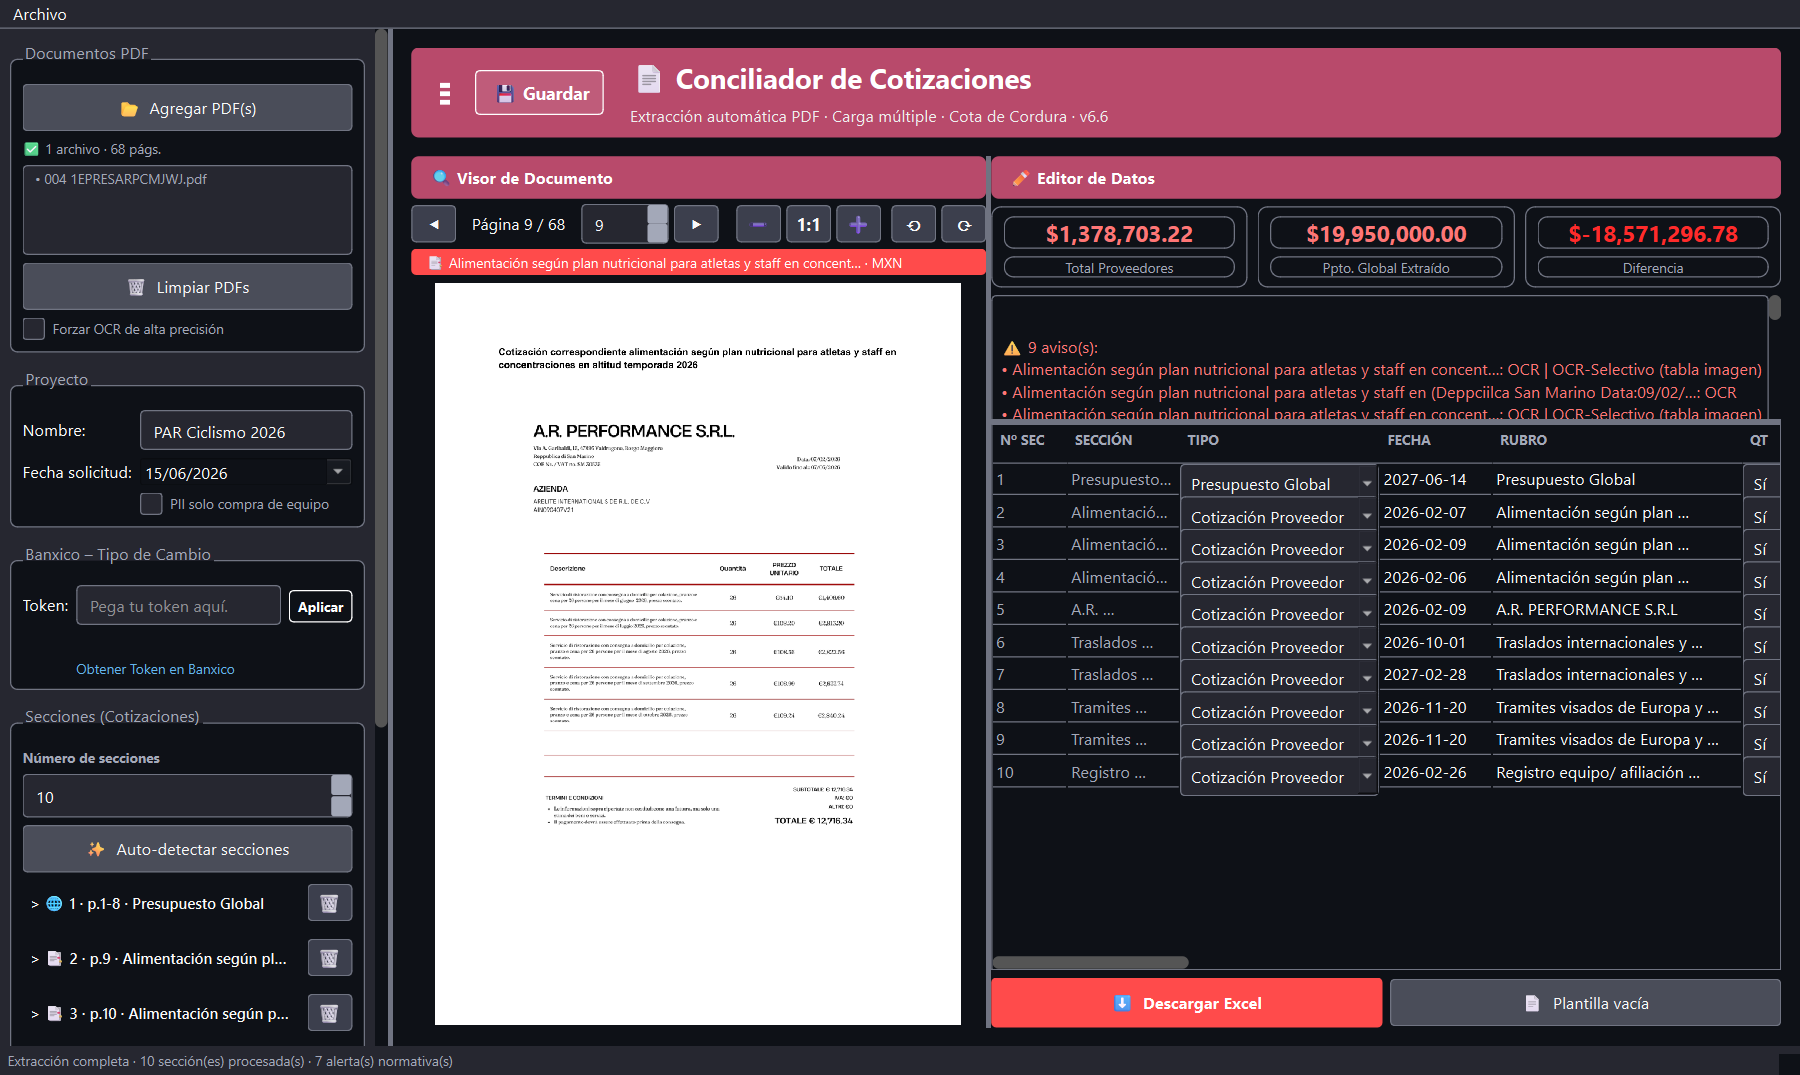
\includegraphics[width=\linewidth, height=0.60\textheight, keepaspectratio]{../images/03_tabla_resultados.png}
    \end{columns}
\end{frame}

% ── Diapositiva 7: Validación Normativa EFIDEPORTE ──
\begin{frame}{Validación Normativa Automatizada (7 Reglas EFIDEPORTE)}
    Auditoría consultiva automática al finalizar la extracción (panel de avisos y barra de estado):

    \vspace{0.3cm}
    \begin{columns}[T]
        \column{0.49\textwidth}
        \begin{enumerate}
            \item \textbf{Vigencia (Regla 2):} Verifica que ninguna cotización supere 90 días respecto a la \textit{Fecha solicitud}.
            \item \textbf{Tope 5\% Admin (Regla 3):} Detecta honorarios de contador, papelería o renta y alerta si exceden el 5\%.
            \item \textbf{Rubros Prohibidos (Regla 10):} Señala conceptos como \textit{imprevistos}, \textit{préstamos} o \textit{ganancia propia}.
            \item \textbf{Duplicados (Regla 10c):} Identifica conceptos iguales con montos similares ($<5\%$ de diferencia).
        \end{enumerate}

        \column{0.49\textwidth}
        \begin{enumerate}
            \setcounter{enumi}{4}
            \item \textbf{Seguro Obligatorio (Regla 1):} Verifica al menos una partida de póliza de seguro del proyecto.
            \item \textbf{PII solo compra de equipo (Regla 3):} Si se marca la casilla en \textit{Proyecto}, alerta de inmediato ante gastos administrativos.
            \item \textbf{Aportación en Especie (Regla e):} Emite recordatorio de CFDI al detectar equipamiento aportado.
        \end{enumerate}

        \vspace{0.25cm}
        \fcolorbox{vino}{vino!8}{
            \parbox{0.94\linewidth}{
                \small\color{vinoDark}\textbf{Carácter consultivo:} Las alertas previenen errores ante la SHCP sin bloquear la edición manual ni la exportación a Excel.
            }
        }
    \end{columns}
\end{frame}

% ── Diapositiva 8: Cierre ──
\begin{frame}
    \begin{columns}[c]
        \column{0.62\textwidth}
        \begin{center}
            {\Huge \textcolor{vino}{\textbf{¡Gracias!}}}\\[0.6cm]
            {\Large \textbf{¿Tienen alguna pregunta?}}\\[0.7cm]
            \normalsize Secretaría de Hacienda y Crédito Público (SHCP)\\
            Unidad de Política e Ingresos Tributarios (UPIT)\\[0.3cm]
            \small\color{vinoDark} Conciliador de Cotizaciones v6.6 · EFIDEPORTE
        \end{center}

        \column{0.34\textwidth}
        \begin{center}
            \fcolorbox{vino!40}{white}{
                \parbox{0.85\linewidth}{
                    \centering
                    \textbf{\footnotesize\color{vino}Buzón de Mejora Continua}\\[4pt]
                    
\includegraphics[width=2.5cm]{../images/qr_formulario.png}\\[4pt]
                    {\scriptsize Reporta incidencias o sugiere mejoras directamente desde el código QR.}
                }
            }
        \end{center}
    \end{columns}
\end{frame}

\end{document}
